\documentclass[letterpaper]{article}

../../../../tex/scufftex.tex

\graphicspath{{figures/}}

%------------------------------------------------------------
%------------------------------------------------------------
%- Special commands for this document -----------------------
%------------------------------------------------------------
%------------------------------------------------------------
\newcommand{\vbEps}{\boldsymbol{\epsilon}}

%------------------------------------------------------------
%------------------------------------------------------------
%- Document header  -----------------------------------------
%------------------------------------------------------------
%------------------------------------------------------------
\title {Scattering Amplitudes from Surface Currents in {\sc scuff-em}}
\author {Homer Reid}
\date {January 22, 2014}


%------------------------------------------------------------
%------------------------------------------------------------
%- Start of actual document
%------------------------------------------------------------
%------------------------------------------------------------

\begin{document}
\pagestyle{myheadings}
\markright{Homer Reid: Scattering Amplitudes from Surface Currents}
\maketitle

\tableofcontents

%%%%%%%%%%%%%%%%%%%%%%%%%%%%%%%%%%%%%%%%%%%%%%%%%%%%%%%%%%%%%%%%%%%%%%
%%%%%%%%%%%%%%%%%%%%%%%%%%%%%%%%%%%%%%%%%%%%%%%%%%%%%%%%%%%%%%%%%%%%%%
%%%%%%%%%%%%%%%%%%%%%%%%%%%%%%%%%%%%%%%%%%%%%%%%%%%%%%%%%%%%%%%%%%%%%%
\newpage 
\section{Compact objects}

First consider a compact scattering geometry (consisting of one or 
more objects) localized near the origin of coordinates and illuminated 
by an arbitrary unspecified external sources at frequency 
$\omega=ck_0$ (i.e. $k_0$ is the free-space wavenumber corresponding
to the frequency at which we work). At large distances, we write the 
scattered electric field in the form
%%%%%%%%%%%%%%%%%%%%%%%%%%%%%%%%%%%%%%%%%%%%%%%%%%%%%%%%%%%%%%%%%%%%%%
\numeq{FDef}
{\vb E\sups{scat}(\vb x) = 
   \vb E\sups{scat}(r,\Omega)
   =\vb F(\Omega) \frac{e^{ikr}}{4\pi r}
}
%%%%%%%%%%%%%%%%%%%%%%%%%%%%%%%%%%%%%%%%%%%%%%%%%%%%%%%%%%%%%%%%%%%%%%
which defines the \textit{scattering amplitude}
$\vb F(\Omega)$; it is a function of solid angle only,
not of the distance from the target to the evaluation point.

On the other hand, we also have the usual expression
for the scattered electric field in terms of the surface
currents,
%%%%%%%%%%%%%%%%%%%%%%%%%%%%%%%%%%%%%%%%%%%%%%%%%%%%%%%%%%%%%%%%%%%%%%
\begin{align*}
 \vb E\sups{scat}(\vb x)
&=\oint \Big\{ \BG\supt{EE}(\vb x,\vb x^\prime)\cdot \vb K(\vb x^\prime)
              +\BG\supt{EM}(\vb x,\vb x^\prime)\cdot \vb N(\vb x^\prime)
        \Big\}d\vb x^\prime
\\
&=ik_0\oint \Big\{ Z_0 Z^r\vb G(\vb x,\vb x^\prime)\cdot \vb K(\vb x^\prime)
                 +\vb C(\vb x,\vb x^\prime)\cdot \vb N(\vb x^\prime)
        \Big\}d\vb x^\prime
\end{align*}
where $k_0$ and $Z^r$ are the wavenumber and relative wave impedance 
of the exterior medium.
%%%%%%%%%%%%%%%%%%%%%%%%%%%%%%%%%%%%%%%%%%%%%%%%%%%%%%%%%%%%%%%%%%%%%%

%%%%%%%%%%%%%%%%%%%%%%%%%%%%%%%%%%%%%%%%%%%%%%%%%%%%%%%%%%%%%%%%%%%%%%
%%%%%%%%%%%%%%%%%%%%%%%%%%%%%%%%%%%%%%%%%%%%%%%%%%%%%%%%%%%%%%%%%%%%%%
%%%%%%%%%%%%%%%%%%%%%%%%%%%%%%%%%%%%%%%%%%%%%%%%%%%%%%%%%%%%%%%%%%%%%%
\newpage
\section{Extended objects}

Next we consider an extended structure described by Bloch-periodic
boundary conditions. We will derive expressions for the 
plane-wave reflection and transmission coefficients in terms
of the surface-current distribution in the unit cell of the structure.

%%%%%%%%%%%%%%%%%%%%%%%%%%%%%%%%%%%%%%%%%%%%%%%%%%%%%%%%%%%%%%%%%%%%%%
%%%%%%%%%%%%%%%%%%%%%%%%%%%%%%%%%%%%%%%%%%%%%%%%%%%%%%%%%%%%%%%%%%%%%%
%%%%%%%%%%%%%%%%%%%%%%%%%%%%%%%%%%%%%%%%%%%%%%%%%%%%%%%%%%%%%%%%%%%%%%
\subsection*{Definition of scattering coefficients}

For definiteness, I suppose that the structure is infinitely 
extended in the $x$ and $y$ directions with finite extent in
the $z$ direction, and I suppose the structure is illuminated 
from below by a plane wave with propagation vector confined
to the $xz$ plane. More general situations could easily be 
handled by extending the methods of this section.

The incident, reflected, and transmitted electric fields
may be written in the form
%%%%%%%%%%%%%%%%%%%%%%%%%%%%%%%%%%%%%%%%%%%%%%%%%%%%%%%%%%%%%%%%%%%%%%
\begin{subequations}
\begin{align}
  \vb E\sups{inc}(\vb x)
&=E_0 \vbEps_0 e^{ i (k_x x + k_z z)}
\\
   \vb E\sups{refl}(\vb x)
&=rE_0 \vbEps_0\sups{refl} e^{ i (k_x x - k_z z)}
\\
  \vb E\sups{trans}(\vb x)
&=tE_0\vbEps_0\sups{trans} e^{ i (k_x x + k_z^\prime z)}
\end{align}
\label{trDef}
\end{subequations}
where $E_0$ is the incident field magnitude and 
$\vbEps_0$ is a polarization vector.
Equations (\ref{trDef}b) and (\ref{trDef}c)
define the reflection and transmission coefficients 
$r$ and $t$. Also, the components of the propagation
vector in the lower medium are 
%%%%%%%%%%%%%%%%%%%%%%%%%%%%%%%%%%%%%%%%%%%%%%%%%%%%%%%%%%%%%%%%%%%%%%
$$ k_x = k_0\sin\theta, \qquad k_z=k_0\cos\theta$$
%%%%%%%%%%%%%%%%%%%%%%%%%%%%%%%%%%%%%%%%%%%%%%%%%%%%%%%%%%%%%%%%%%%%%%
(where $\theta$ is the incident angle of the illuminating
radiation) and 
%%%%%%%%%%%%%%%%%%%%%%%%%%%%%%%%%%%%%%%%%%%%%%%%%%%%%%%%%%%%%%%%%%%%%%
\numeq{kzPrime1}{k_z^\prime = \sqrt{ k_0^{\prime 2} - k_x^2}}
where 
%%%%%%%%%%%%%%%%%%%%%%%%%%%%%%%%%%%%%%%%%%%%%%%%%%%%%%%%%%%%%%%%%%%%%%
$$ k_0^\prime = \sqrt{\epsilon^\prime \mu^\prime}\cdot k_0$$
%%%%%%%%%%%%%%%%%%%%%%%%%%%%%%%%%%%%%%%%%%%%%%%%%%%%%%%%%%%%%%%%%%%%%%
is the wavenumber in the upper medium.

\subsubsection*{TE and TM Polarizations} 

For the TE polarization, the polarization vectors in 
(\ref{trDef}) are all equal:
%%%%%%%%%%%%%%%%%%%%%%%%%%%%%%%%%%%%%%%%%%%%%%%%%%%%%%%%%%%%%%%%%%%%%%
\begin{align*}
 \text{TE:} 
   \qquad \vbEps_0&=\vbEps_0\sups{refl}=\vbEps_0\sups{trans}=\vbhat{y}.
\\
 \text{TM:} 
   \qquad \vbEps_0&=\cos\theta\,\vbhat{x} - \sin\theta\,\vbhat{z} \\
 \vbEps\sups{refl}&=\cos\theta\,\vbhat{x} + \sin\theta\,\vbhat{z} \\
\vbEps\sups{trans}&=\cos\theta^\prime \, \vbhat{x} - \sin\theta^\prime\vbhat{z}
\end{align*}
where 
$$\sin\theta^\prime = \sqrt\frac{1}{\epsilon^\prime \mu^\prime} 
  \sin\theta.
$$
%%%%%%%%%%%%%%%%%%%%%%%%%%%%%%%%%%%%%%%%%%%%%%%%%%%%%%%%%%%%%%%%%%%%%%

\subsubsection*{Bloch periodicity} 

Notice that all fields satisfy Bloch-periodic boundary conditions,
\numeq{BlochPeriodicity1}
{\vb E(\vb x+\vb L) = e^{i\vb k \cdot \vb L}\,\vb E(\vb x)}
where the Bloch wavevector is 
$$\vb k=k_0 \sin\theta \, \vbhat{x}.$$
For the plane waves (\ref{trDef}), equation (\ref{BlochPeriodicity1})
actually holds for any arbitrary vector $\vb L$; for our 
purposes we will only need to use it for certain special
vectors $\vb L$ determined by the structure of the lattice in
our PBC geometry.

%%%%%%%%%%%%%%%%%%%%%%%%%%%%%%%%%%%%%%%%%%%%%%%%%%%%%%%%%%%%%%%%%%%%%%
%%%%%%%%%%%%%%%%%%%%%%%%%%%%%%%%%%%%%%%%%%%%%%%%%%%%%%%%%%%%%%%%%%%%%%
%%%%%%%%%%%%%%%%%%%%%%%%%%%%%%%%%%%%%%%%%%%%%%%%%%%%%%%%%%%%%%%%%%%%%%
\subsection*{Fields from surface currents}

On the other hand, the scattered $\vb E$ fields in the uppermost
and lowermost regions may be obtained in the usual way from the
surface-current distributions on the surfaces bounding those
regions. For example, at points in the upper medium we have 
%%%%%%%%%%%%%%%%%%%%%%%%%%%%%%%%%%%%%%%%%%%%%%%%%%%%%%%%%%%%%%%%%%%%%%
\begin{align}
 \vb E\sups{trans}(\vb x)
&=\oint_{\mc S} \Big\{ 
   \BG\supt{EE}(\vb x,\vb x^\prime)\cdot \vb K(\vb x^\prime)
  +\BG\supt{EM}(\vb x,\vb x^\prime)\cdot \vb N(\vb x^\prime)
                \Big\}d\vb x^\prime
\nn
&=ik_0^\prime \oint_{\mc S} \Big\{ 
   Z_0 Z^\prime \vb G(k_0^\prime; \vb x,\vb x^\prime)
                    \cdot \vb K(\vb x^\prime)
               +\vb C(k_0^\prime; \vb x,\vb x^\prime)
                    \cdot \vb N(\vb x^\prime) \Big\}d\vb x^\prime
\label{ETransPBC}
\end{align}
%%%%%%%%%%%%%%%%%%%%%%%%%%%%%%%%%%%%%%%%%%%%%%%%%%%%%%%%%%%%%%%%%%%%%%
where $\mc S$ is the surface bounding the uppermost medium and
$k_0^\prime, Z^\prime$ are the wavenumber and relative wave 
impedance of the uppermost region:
%%%%%%%%%%%%%%%%%%%%%%%%%%%%%%%%%%%%%%%%%%%%%%%%%%%%%%%%%%%%%%%%%%%%%%
$$k_0^\prime=\sqrt{\epsilon^\prime \mu^\prime }\cdot \vb k_0,
  \qquad
  Z^\prime=\sqrt{\frac{\mu^\prime}{\epsilon^\prime}}.
$$
%%%%%%%%%%%%%%%%%%%%%%%%%%%%%%%%%%%%%%%%%%%%%%%%%%%%%%%%%%%%%%%%%%%%%%
Using the Bloch-periodicity of the surface currents, i.e.
%%%%%%%%%%%%%%%%%%%%%%%%%%%%%%%%%%%%%%%%%%%%%%%%%%%%%%%%%%%%%%%%%%%%%%
$$ \left\{ \begin{array}{c} 
   \vb K(\vb x+\vb L) \\[5pt] \vb N(\vb x+\vb L)
   \end{array}\right\}
   =
   e^{i\vb k \cdot \vb L}
   \left\{ \begin{array}{c} 
   \vb K(\vb x) \\[5pt] \vb N(\vb x)
   \end{array}\right\}
$$
%%%%%%%%%%%%%%%%%%%%%%%%%%%%%%%%%%%%%%%%%%%%%%%%%%%%%%%%%%%%%%%%%%%%%%
we can restrict the surface integral in (\ref{ETransPBC}) to 
just the lattice unit cell:
%%%%%%%%%%%%%%%%%%%%%%%%%%%%%%%%%%%%%%%%%%%%%%%%%%%%%%%%%%%%%%%%%%%%%%
\numeq{EIntegralUnitCell}
{
 \vb E\sups{trans}(\vb x)
=ik_0^\prime \int_{U} 
  \Big\{
  Z_0 Z^\prime 
   \overline{\vb G}(k_0^\prime; \vb x, \vb x^\prime) \cdot \vb K(\vb x^\prime)
  +\overline{\vb C}(k_0^\prime; \vb x, \vb x^\prime) \cdot \vb N(\vb x^\prime)
  \Big\}\,d\vb x^\prime
}
%%%%%%%%%%%%%%%%%%%%%%%%%%%%%%%%%%%%%%%%%%%%%%%%%%%%%%%%%%%%%%%%%%%%%%
where the periodic Green's functions are
\numeq{PeriodicGFs}
{
   \left\{ \begin{array}{c} 
   \overline{\vb G}(\vb x, \vb x^\prime) \\[5pt]
   \overline{\vb C}(\vb x, \vb x^\prime)
   \end{array}\right\}
   \equiv 
   \sum_{\vb L} e^{i\vb k \cdot \vb L}
   \left\{ \begin{array}{c}
   \vb G(\vb x, \vb x^\prime+\vb L) \\[5pt]
   \vb C(\vb x, \vb x^\prime+\vb L)
   \end{array}\right\}
}
%%%%%%%%%%%%%%%%%%%%%%%%%%%%%%%%%%%%%%%%%%%%%%%%%%%%%%%%%%%%%%%%%%%%%%
I now invoke the following representation of the dyadic 
Green's functions (Chew, 1995): for $z>z^\prime$,
%%%%%%%%%%%%%%%%%%%%%%%%%%%%%%%%%%%%%%%%%%%%%%%%%%%%%%%%%%%%%%%%%%%%%%
\begin{subequations}
\begin{align}
 \vb G(k_0^\prime; \vbrho, z; \vbrho^\prime, z^\prime)
&=\frac{i}{2} 
  \, 
  \int \frac{d\vb q}{(2\pi)^2 q_z}
  \, 
  \vbhat{G}(\vb q) e^{i\vb q\cdot (\vbrho-\vbrho^\prime)}
                   e^{iq_z(z-z^\prime)}
\\
 \vb C(k_0^\prime; \vbrho, z; \vbrho^\prime, z^\prime)
&=\frac{i}{2} 
  \, 
  \int \frac{d\vb q}{(2\pi)^2 q_z}
  \, 
  \vbhat{C}(\vb q) e^{i\vb q\cdot (\vbrho-\vbrho^\prime)}
                   e^{iq_z(z-z^\prime)}
\end{align}
\label{SpectralGFs}
\end{subequations}
where $\vb q=(q_x,q_y)$ is a two-dimensional Fourier wavevector,
$d\vb q=dq_x dq_y$,
$q_z=\sqrt{k_0^{\prime 2}-|\vb q|^2}$, and 
%%%%%%%%%%%%%%%%%%%%%%%%%%%%%%%%%%%%%%%%%%%%%%%%%%%%%%%%%%%%%%%%%%%%%%
\begin{align*}
 \vbhat{G}(\vb q)
   &=\left(\begin{array}{ccc}
      1 & 0 & 0 \\ 
      0 & 1 & 0 \\ 
      0 & 0 & 1
     \end{array}\right)
     -\frac{1}{k_0^{\prime 2}}
     \left(\begin{array}{ccc}
      q_x^2   & q_x q_y & q_x q_z \\
      q_yq_x  & q_y^2   & q_y q_z \\
      q_z q_x & q_z q_y & q_z^2
     \end{array}\right)
\\
 \vbhat{C}(\vb q)
   &=\frac{1}{k_0^\prime}
     \left(\begin{array}{ccc}
       0 & q_z & -q_y \\
    -q_z &   0 &  q_x \\
     q_y &-q_x &    0
     \end{array}\right).
\end{align*}
%%%%%%%%%%%%%%%%%%%%%%%%%%%%%%%%%%%%%%%%%%%%%%%%%%%%%%%%%%%%%%%%%%%%%%
Inserting (\ref{SpectralGFs}) into (\ref{PeriodicGFs}), I 
obtain, for the periodic version of e.g. the $\vb G$ kernel,
%%%%%%%%%%%%%%%%%%%%%%%%%%%%%%%%%%%%%%%%%%%%%%%%%%%%%%%%%%%%%%%%%%%%%%
\begin{align*}
\overline{\vb G}(k_0^\prime; \vbrho, z; \vbrho^\prime, z)
&=\frac{i}{2}\int \frac{d\vb q}{(2\pi)^2 q_z}
  \vbhat{G}(\vb q) e^{i\vb q \cdot (\vbrho - \vbrho^\prime)}
   e^{iq_z(z-z^\prime)}
  \underbrace{\sum_{\vb L} e^{i(\vb k - \vb q) \cdot \vb L}}
             _{\mc V^{-1} \delta(\vb k-\vb q)}
\end{align*}
%%%%%%%%%%%%%%%%%%%%%%%%%%%%%%%%%%%%%%%%%%%%%%%%%%%%%%%%%%%%%%%%%%%%%%
The sum over lattice vectors $\vb L$ yields a two-dimensional
$\delta$ function whose prefactor is $\mc V$, the volume
of the lattice unit cell.\footnote{A more precise statement
would be that the sum over lattice vectors defines a 
\textit{train} of $\delta$ functions,
$$ \sum_{\vb L} e^{i(\vb k - \vb q) \cdot \vb L}
   =\frac{1}{\mc V} \sum_{\BG} \delta(\vb k - \vb q - \BG)
$$ 
where the sum is over reciprocal lattice vectors. In
the above we have truncated this sum at the term
$\BG=0$, which is justified for evaluating fields
at large distance from the surface because the 
$\BG\ne 0$ terms will typically correspond to 
evanescent waves.} Using this to evaluate the $\vb q$
integrals in (\ref{SpectralGFs}) yields
%====================================================================%
\numeq{OverlineGC}
{ \left\{ \begin{array}{c} 
    \overline{\vb G}(k_0^\prime; \vbrho, z; \vbrho^\prime, z)
    \\[5pt]
    \overline{\vb C}(k_0^\prime; \vbrho, z; \vbrho^\prime, z)
    \end{array}\right\}
  =\frac{i}{2 \mc V k^\prime_z}
   \left\{ \begin{array}{c}
     \vbhat{G}(\vb k) \\[5pt] \vbhat{C}(\vb k)
   \end{array}\right\}
   e^{i\vb k \cdot (\vbrho - \vbrho^\prime)}
   e^{ik^\prime_z(z-z^\prime)}
}
%====================================================================%
where $k^\prime_z$ is defined in terms of the wavenumber 
$k_0^\prime$ and the Bloch wavevector $\vb k$ by
%====================================================================%
$$ k^\prime_z = \sqrt{k_0^{\prime 2} - |\vb k|^2}.$$
%====================================================================%
[This is the same equation as (\ref{kzPrime1}).]
Inserting (\ref{OverlineGC}) into (\ref{EIntegralUnitCell}), 
the scattered field above the surface takes the form
%====================================================================%
\begin{align}
 &\hspace{-0.05in} \vb E\sups{trans}(\vb x)
\nn
&=
 e^{i(k_x x + k_z^\prime z)}
        \left\{ -\frac{k_0^\prime}{2\mc V k_z^\prime}
        \int_U e^{-i(\vb k \cdot \vbrho^\prime + k_z z^\prime)}
        \left[ Z_0 Z^\prime \vbhat{G}(\vb k)\cdot \vb K(\vb x^\prime)
                +\vbhat{C}(\vb k)\cdot \vb N(\vb x^\prime)
        \right] \, d\vb x^\prime
        \right\}
\label{ETransSurfaceIntegral}
\end{align}
%====================================================================%

\subsection*{Transmission coefficient for TE polarization}

%%%%%%%%%%%%%%%%%%%%%%%%%%%%%%%%%%%%%%%%%%%%%%%%%%%%%%%%%%%%%%%%%%%%%%
\begin{align*}
 t\supt{TE}
&=-\frac{k_0^\prime}{2 \mc V k_z^\prime}
   \int_U e^{-i(\vb k \cdot \vbrho^\prime + k_z z^\prime)}
        \left[ Z_0 Z^\prime 
               (\vbEps_0\sups{trans})^\dagger \cdot 
               \vbhat{G}(\vb k) \cdot \vb K(\vb x^\prime)
               +(\vbEps_0\sups{trans})^\dagger \cdot 
               \vbhat{C}(\vb k)\cdot \vb N(\vb x^\prime) 
        \right] \, d\vb x^\prime
\end{align*}
%%%%%%%%%%%%%%%%%%%%%%%%%%%%%%%%%%%%%%%%%%%%%%%%%%%%%%%%%%%%%%%%%%%%%%
We have 
%%%%%%%%%%%%%%%%%%%%%%%%%%%%%%%%%%%%%%%%%%%%%%%%%%%%%%%%%%%%%%%%%%%%%%
\begin{align*}
&\hspace{-0.05in}
 (\vbEps_0\sups{trans})^\dagger \cdot
 \vbhat{G}(\vb k) \cdot \vb K(\vb x^\prime)
\\
&=
 \left(\begin{array}{c}0 \\ 1 \\ 0\end{array}\right)^\dagger
 \left[ \left(\begin{array}{ccc}
               1 & 0 & 0 \\ 
               0 & 1 & 0 \\ 
               0 & 0 & 1
              \end{array}\right)
       -\frac{1}{k_0^{\prime 2}}
        \left(\begin{array}{ccc}
               k_x^2   & k_x k_y & k_x k_z \\
               k_yk_x  & k_y^2   & k_y k_z \\
               k_z k_x & k_z k_y & k_z^2
              \end{array}
        \right)
 \right]
 \left(\begin{array}{c}K_x \\ K_y \\ K_z\end{array}\right)
\\
&=
 \frac{1}{k_0^{\prime 2}}
 \left(\begin{array}{c}0 \\ 1 \\ 0\end{array}\right)^\dagger
 \left(\begin{array}{c} -k_y k_x K_x \\ (k_0^{\prime 2}-k_y^2)K_y \\ -k_y k_z K_z
       \end{array}\right)
\\
&= K_y
\end{align*}
since, in our setup, the $y$ component of the Bloch 
wavevector is $k_y=0.$

Similarly, 
%%%%%%%%%%%%%%%%%%%%%%%%%%%%%%%%%%%%%%%%%%%%%%%%%%%%%%%%%%%%%%%%%%%%%%
\begin{align*}
&\hspace{-0.05in}
 (\vbEps_0\sups{trans})^\dagger \cdot
 \vbhat{C}(\vb k) \cdot \vb N(\vb x^\prime)
\\
&=
 \left(\begin{array}{c}0 \\ 1 \\ 0\end{array}\right)^\dagger
 \left[ \frac{1}{k_0^{\prime}}
        \left(\begin{array}{ccc}
               0       & k_z     & -k_y    \\
               -k_z    & 0       & k_x     \\
               k_y     & -k_x    & 0
              \end{array}
        \right)
 \right]
 \left(\begin{array}{c}N_x \\ N_y \\ N_z\end{array}\right)
\\
&=
 \frac{1}{k_0^\prime}
 \left(\begin{array}{c}0 \\ 1 \\ 0\end{array}\right)^\dagger
 \left(\begin{array}{c} \cdots \\ -k_z N_x + k_x N_z \\ \cdots
       \end{array}\right)
\\
&=-\cos\theta^\prime N_x + \sin\theta^\prime N_z.
\end{align*}
%%%%%%%%%%%%%%%%%%%%%%%%%%%%%%%%%%%%%%%%%%%%%%%%%%%%%%%%%%%%%%%%%%%%%%
Putting it all together, 
%%%%%%%%%%%%%%%%%%%%%%%%%%%%%%%%%%%%%%%%%%%%%%%%%%%%%%%%%%%%%%%%%%%%%%
\begin{align*}
 t\supt{TE}
&=-\frac{k_0^\prime}{2\mc V k_z^\prime}
   \int_U e^{-i(\vb k \cdot \vbrho^\prime + k_z z^\prime)}
        \Big[ Z_0 Z^\prime K_y(\vb x^\prime)
               -\cos\theta^\prime N_x(\vb x^\prime)
               +\sin\theta^\prime N_z(\vb x^\prime)
        \Big] \, d\vb x^\prime
\\
&=-\frac{1}{2\mc V}
   \int_U e^{-i(\vb k \cdot \vbrho^\prime + k_z z^\prime)}
        \Big[ Z_0 Z^\prime 
              \frac{ K_y(\vb x^\prime)}{\cos\theta^\prime}
                    -N_x(\vb x^\prime)
                    +\tan\theta^\prime N_z(\vb x^\prime)
        \Big] \, d\vb x^\prime....
\end{align*}
%%%%%%%%%%%%%%%%%%%%%%%%%%%%%%%%%%%%%%%%%%%%%%%%%%%%%%%%%%%%%%%%%%%%%%

\subsection*{Transmission coefficient for TM polarization}

%%%%%%%%%%%%%%%%%%%%%%%%%%%%%%%%%%%%%%%%%%%%%%%%%%%%%%%%%%%%%%%%%%%%%%
\begin{align*}
 t\supt{TM}
&=-\frac{k_0^\prime}{2 \mc V k_z^\prime}
   \int_U e^{-i(\vb k \cdot \vbrho^\prime + k_z z^\prime)}
        \left[ Z_0 Z^\prime 
               (\vbEps_0\sups{trans})^\dagger \cdot 
               \vbhat{G}(\vb k) \cdot \vb K(\vb x^\prime)
               +(\vbEps_0\sups{trans})^\dagger \cdot 
               \vbhat{C}(\vb k)\cdot \vb N(\vb x^\prime) 
        \right] \, d\vb x^\prime
\end{align*}
%%%%%%%%%%%%%%%%%%%%%%%%%%%%%%%%%%%%%%%%%%%%%%%%%%%%%%%%%%%%%%%%%%%%%%
We have 
%%%%%%%%%%%%%%%%%%%%%%%%%%%%%%%%%%%%%%%%%%%%%%%%%%%%%%%%%%%%%%%%%%%%%%
\begin{align*}
&\hspace{-0.05in}
 (\vbEps_0\sups{trans})^\dagger \cdot
 \vbhat{G}(\vb k) \cdot \vb K(\vb x^\prime)
\\
\\&=
 \left(\begin{array}{c}\cos\theta^\prime \\ 0 \\-\sin\theta^\prime \end{array}\right)^\dagger
 \left[ \left(\begin{array}{ccc}
               1 & 0 & 0 \\ 
               0 & 1 & 0 \\ 
               0 & 0 & 1
              \end{array}\right)
       -\frac{1}{k_0^{\prime 2}}
        \left(\begin{array}{ccc}
               k_x^2   & k_x k_y & k_x k_z \\
               k_yk_x  & k_y^2   & k_y k_z \\
               k_z k_x & k_z k_y & k_z^2
              \end{array}
        \right)
 \right]
 \left(\begin{array}{c}K_x \\ K_y \\ K_z\end{array}\right)
\intertext{Use $\cos\theta^\prime=k_z/k_0^\prime$, 
               $\sin\theta^\prime=k_x/k_0^\prime$:}
&=
 \cos\theta^\prime K_x - \sin\theta^\prime K_z
\end{align*}
%%%%%%%%%%%%%%%%%%%%%%%%%%%%%%%%%%%%%%%%%%%%%%%%%%%%%%%%%%%%%%%%%%%%%%
\begin{align*}
&\hspace{-0.05in}
 (\vbEps_0\sups{trans})^\dagger \cdot
 \vbhat{C}(\vb k) \cdot \vb N(\vb x^\prime)
\\
&=
 \left(\begin{array}{c}\cos\theta^\prime \\ 0 \\-\sin\theta^\prime \end{array}\right)^\dagger
 \left[ \frac{1}{k_0^{\prime}}
        \left(\begin{array}{ccc}
               0       & k_z     & -k_y    \\
               -k_z    & 0       & k_x     \\
               k_y     & -k_x    & 0
              \end{array}
        \right)
 \right]
 \left(\begin{array}{c}N_x \\ N_y \\ N_z\end{array}\right)
\\
&=
 N_y.
\end{align*}
%%%%%%%%%%%%%%%%%%%%%%%%%%%%%%%%%%%%%%%%%%%%%%%%%%%%%%%%%%%%%%%%%%%%%%
Putting it all together, 
%%%%%%%%%%%%%%%%%%%%%%%%%%%%%%%%%%%%%%%%%%%%%%%%%%%%%%%%%%%%%%%%%%%%%%
\begin{align*}
 t\supt{TM}
&=-\frac{1}{2\mc V}
   \int_U e^{-i(\vb k \cdot \vbrho^\prime + k_z z^\prime)}
        \Big[  Z_0 Z^\prime K_x(\vb x^\prime)
              -\tan\theta^\prime Z_0 Z^\prime K_z(\vb x^\prime)
              +\cos\theta^\prime N_y(\vb x^\prime)
        \Big] \, d\vb x^\prime.
\end{align*}
%%%%%%%%%%%%%%%%%%%%%%%%%%%%%%%%%%%%%%%%%%%%%%%%%%%%%%%%%%%%%%%%%%%%%%


\subsection*{Transmission coefficients from surface-current coefficients}

%%%%%%%%%%%%%%%%%%%%%%%%%%%%%%%%%%%%%%%%%%%%%%%%%%%%%%%%%%%%%%%%%%%%%%
$$ \vb K(\vb x)=\sum k_\alpha \vb b_\alpha(\vb x), \qquad 
   \vb N(\vb x)=-Z_0 \sum n_\alpha \vb b_\alpha(\vb x)
$$
%%%%%%%%%%%%%%%%%%%%%%%%%%%%%%%%%%%%%%%%%%%%%%%%%%%%%%%%%%%%%%%%%%%%%%
\begin{align*}
 t\supt{TE}
&=-\frac{Z_0}{2\mc V} \sum_{\alpha}
   \Big[ k_\alpha \frac{Z^\prime}{\cos\theta^\prime} B_{\alpha y}
        +n_\alpha B_{\alpha x} - n_\alpha \tan\theta^\prime B_{\alpha z}.
   \Big]
\\
 t\supt{TM}
&=-\frac{Z_0}{2\mc V} \sum_{\alpha}
   \Big[ k_\alpha Z^\prime B_{\alpha x}
        -k_\alpha Z^\prime \tan\theta^\prime B_{\alpha z}
        -n_\alpha \cos\theta^\prime B_{\alpha y}
   \Big]
\end{align*}
%%%%%%%%%%%%%%%%%%%%%%%%%%%%%%%%%%%%%%%%%%%%%%%%%%%%%%%%%%%%%%%%%%%%%%
where $\vb B_\alpha$ describes an integral over basis functions:
$$ \vb B_\alpha
   \equiv 
   \int_{\sup \vb b_\alpha}
   e^{-i\vb k \cdot \vb x} \, \vb b_\alpha(\vb x)d\vb x.
$$
For RWG functions this integral may be evaluated in closed form:
\begin{align*}
 \vb B_\alpha
&=\ell_\alpha
  \int_0^1 \, du \int_0^u \, dv \,
  \bigg\{
  e^{-i\vb k\cdot [\vb Q^+ + u \vb A^+ + v\vb B]}
  \Big(u\vb A^+ + v\vb B\Big)
\\ 
  &\hspace{1.5in}
  - 
  e^{-i\vb k\cdot [\vb Q^- + u \vb A^- + v\vb B]}
  \Big(u\vb A^- + v\vb B\Big)
  \bigg\}
\\
&=\ell_\alpha\bigg\{ 
  e^{-i\vb k \cdot \vb Q^+} 
  \Big[ f_1\big(\vb k\cdot \vb A^+, \vb k\cdot \vb B\Big) \vb A^+
       +f_2\big(\vb k\cdot \vb A^+, \vb k\cdot \vb B\Big) \vb B
  \Big]
\\
&\qquad \qquad\qquad\qquad\qquad
  -
  e^{-i\vb k \cdot \vb Q^-} 
  \Big[ f_1\big(\vb k\cdot \vb A^-, \vb k\cdot \vb B\Big) \vb A^-
       +f_2\big(\vb k\cdot \vb A^-, \vb k\cdot \vb B\Big) \vb B
  \Big]\bigg\}
\\
\end{align*}
where
\begin{align*}
 f_1(x, y)&=\int_0^1 \, \int_0^u \, u e^{-i (ux + vy)} \,dv\,du  
\\
 f_2(x, y)&=\int_0^1 \, \int_0^u \, v e^{-i (ux + vy)} \,dv\,du  
\end{align*}

\newpage

%####################################################################%
\begin{figure}[H]
\begin{center}
\resizebox{\textwidth}{!}{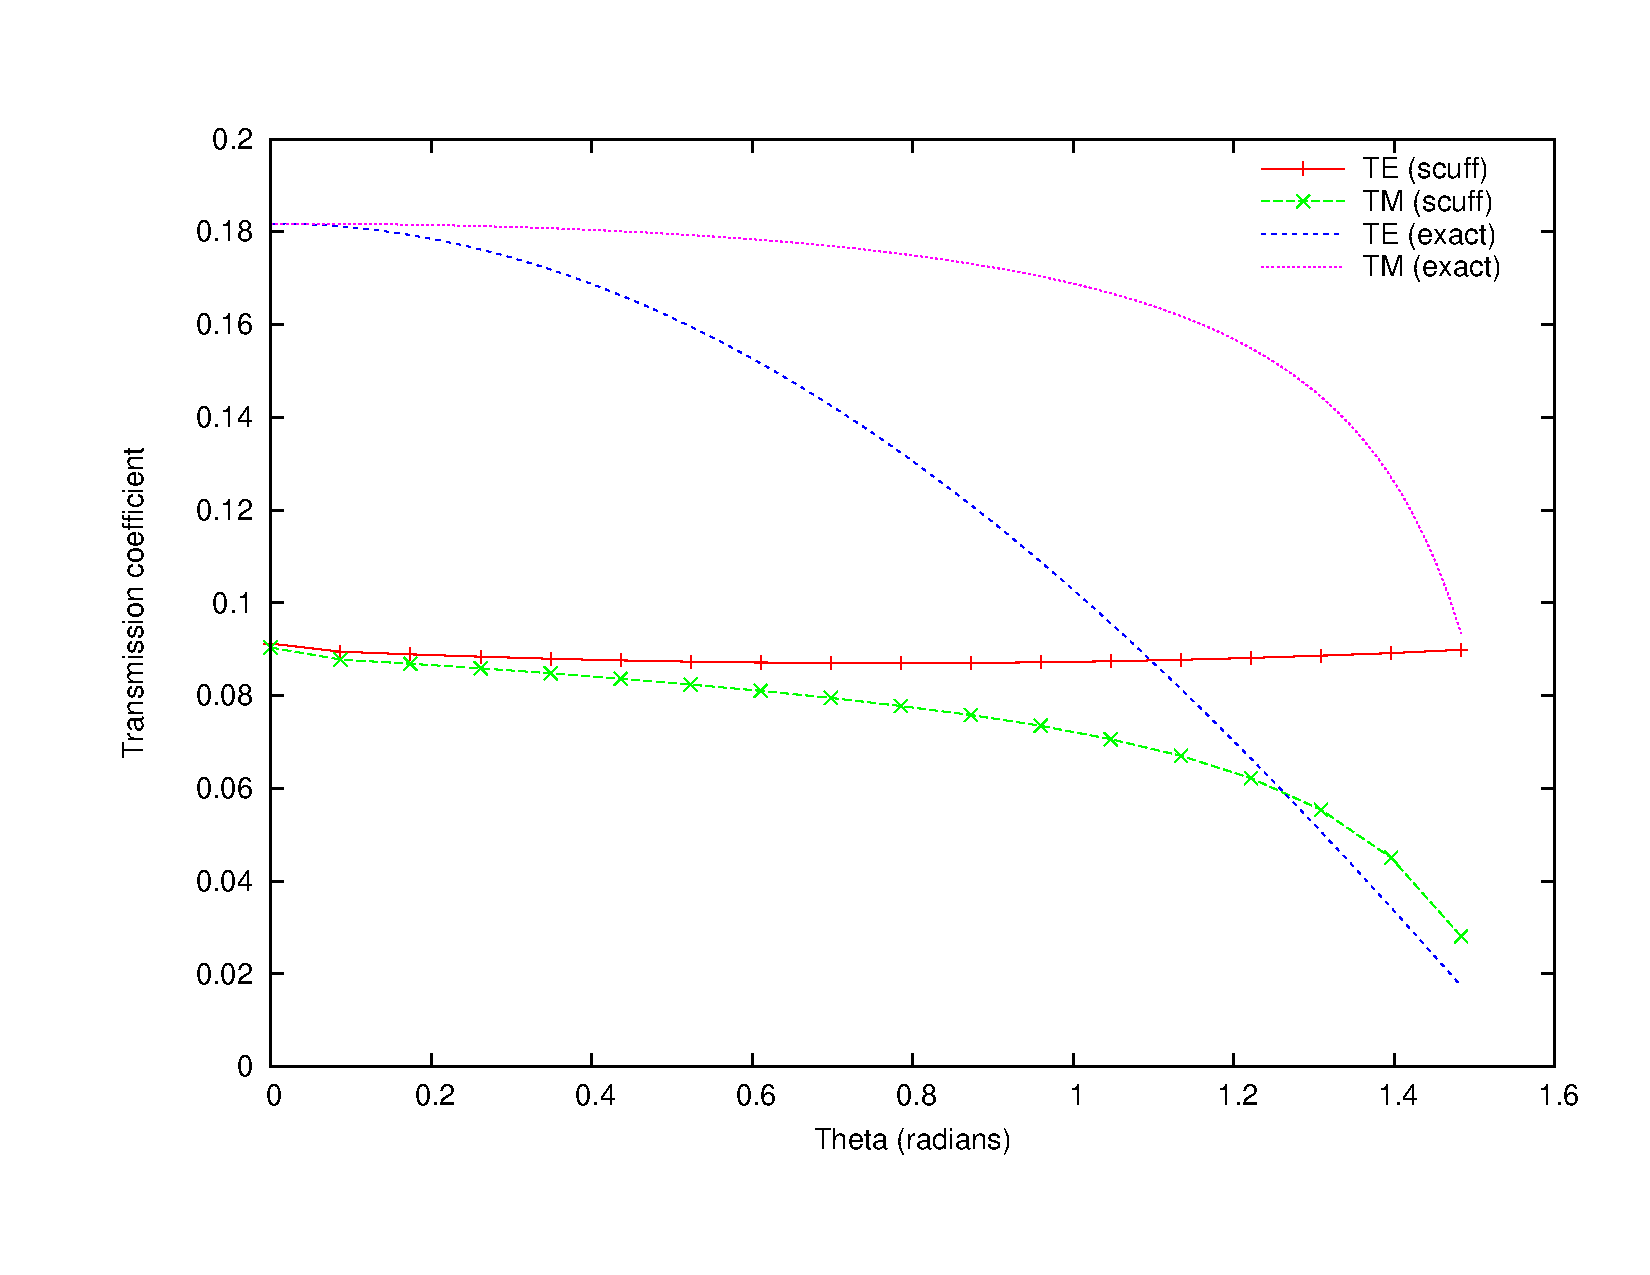
\includegraphics{/home/homer/work/scuff-em-sandbox/TransmissionAmplitudes/scuffFresnel.pdf}}
\caption{Transmission amplitudes vs. incident angle 
         for Fresnel scattering (plane-wave transmission) 
         into a dielectric half-space with $\epsilon^\prime=100.$
        }
\label{PendulumFigure}
\end{center}
\end{figure}
%####################################################################%

\end{document} 
